% Options for packages loaded elsewhere
\PassOptionsToPackage{unicode}{hyperref}
\PassOptionsToPackage{hyphens}{url}
%
\documentclass[
]{article}
\usepackage{amsmath,amssymb}
\usepackage{iftex}
\ifPDFTeX
  \usepackage[T1]{fontenc}
  \usepackage[utf8]{inputenc}
  \usepackage{textcomp} % provide euro and other symbols
\else % if luatex or xetex
  \usepackage{unicode-math} % this also loads fontspec
  \defaultfontfeatures{Scale=MatchLowercase}
  \defaultfontfeatures[\rmfamily]{Ligatures=TeX,Scale=1}
\fi
\usepackage{lmodern}
\ifPDFTeX\else
  % xetex/luatex font selection
\fi
% Use upquote if available, for straight quotes in verbatim environments
\IfFileExists{upquote.sty}{\usepackage{upquote}}{}
\IfFileExists{microtype.sty}{% use microtype if available
  \usepackage[]{microtype}
  \UseMicrotypeSet[protrusion]{basicmath} % disable protrusion for tt fonts
}{}
\makeatletter
\@ifundefined{KOMAClassName}{% if non-KOMA class
  \IfFileExists{parskip.sty}{%
    \usepackage{parskip}
  }{% else
    \setlength{\parindent}{0pt}
    \setlength{\parskip}{6pt plus 2pt minus 1pt}}
}{% if KOMA class
  \KOMAoptions{parskip=half}}
\makeatother
\usepackage{xcolor}
\usepackage{graphicx}
\makeatletter
\def\maxwidth{\ifdim\Gin@nat@width>\linewidth\linewidth\else\Gin@nat@width\fi}
\def\maxheight{\ifdim\Gin@nat@height>\textheight\textheight\else\Gin@nat@height\fi}
\makeatother
% Scale images if necessary, so that they will not overflow the page
% margins by default, and it is still possible to overwrite the defaults
% using explicit options in \includegraphics[width, height, ...]{}
\setkeys{Gin}{width=\maxwidth,height=\maxheight,keepaspectratio}
% Set default figure placement to htbp
\makeatletter
\def\fps@figure{htbp}
\makeatother
\setlength{\emergencystretch}{3em} % prevent overfull lines
\providecommand{\tightlist}{%
  \setlength{\itemsep}{0pt}\setlength{\parskip}{0pt}}
\setcounter{secnumdepth}{-\maxdimen} % remove section numbering
\ifLuaTeX
  \usepackage{selnolig}  % disable illegal ligatures
\fi
\usepackage{bookmark}
\IfFileExists{xurl.sty}{\usepackage{xurl}}{} % add URL line breaks if available
\urlstyle{same}
\hypersetup{
  hidelinks,
  pdfcreator={LaTeX via pandoc}}

\author{}
\date{}

\begin{document}

\hfill\break
Main\_menu.vi\\

\includegraphics{LVtemp20240312184737_0_0c.png}\\
The main menu function acts as the focal point for navigating and
utilizing the diverse range of features and capabilities within our
application. When users initiate the application, they encounter a
user-friendly menu interface, offering a variety of options that cater
to their specific requirements.\\
Key functionalities include:\\
Initiating window plots for data visualization\\
Establishing communication with microcontrollers\\
Implementing robust error handling mechanisms\\
\strut \\
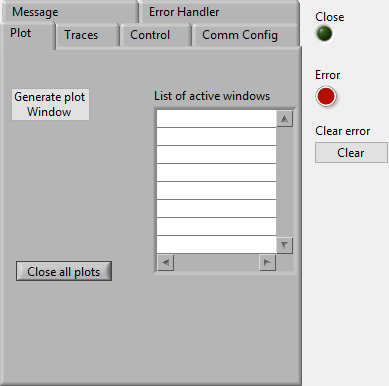
\includegraphics{LVtemp20240312184737_1_0.png}\\
\strut \\

\includegraphics{Clear_Errors_viLVtemp20240312184737_2_0.png}
\textbf{Clear Errors.vi\\
} C:\textbackslash Program Files\textbackslash National
Instruments\textbackslash LabVIEW
2022\textbackslash vi.lib\textbackslash Utility\textbackslash error.llb\textbackslash Clear
Errors.vi\\

\includegraphics{Fc_Get_TRACEDATA_viLVtemp20240312184737_3_0.png}
\textbf{Fc\_Get\_TRACEDATA.vi\\
}
C:\textbackslash Users\textbackslash v\_hernandez\textbackslash Documents\textbackslash Projects\textbackslash C2\textbackslash lrs-soc\textbackslash labview\textbackslash dev\_labview\textbackslash Fc\_Get\_TRACEDATA.vi\\

\includegraphics{Fc_new_plot_viLVtemp20240312184737_4_0.png}
\textbf{Fc\_new\_plot.vi\\
}
C:\textbackslash Users\textbackslash v\_hernandez\textbackslash Documents\textbackslash Projects\textbackslash C2\textbackslash lrs-soc\textbackslash labview\textbackslash dev\_labview\textbackslash Fc\_new\_plot.vi\\

\includegraphics{Fc_receiver_queue_Main_menu_viLVtemp20240312184737_5_0.png}
\textbf{Fc\_receiver\_queue\_Main\_menu.vi\\
}
C:\textbackslash Users\textbackslash v\_hernandez\textbackslash Documents\textbackslash Projects\textbackslash C2\textbackslash lrs-soc\textbackslash labview\textbackslash dev\_labview\textbackslash Fc\_receiver\_queue\_Main\_menu.vi\\

\includegraphics{Fc_save_conf_to_uc_viLVtemp20240312184737_6_0.png}
\textbf{Fc\_save\_conf\_to\_uc.vi\\
}
C:\textbackslash Users\textbackslash v\_hernandez\textbackslash Documents\textbackslash Projects\textbackslash C2\textbackslash lrs-soc\textbackslash labview\textbackslash dev\_labview\textbackslash Fc\_save\_conf\_to\_uc.vi\\

\includegraphics{Fc_SaveCTRLparams_viLVtemp20240312184737_7_0.png}
\textbf{Fc\_SaveCTRLparams.vi\\
}
C:\textbackslash Users\textbackslash v\_hernandez\textbackslash Documents\textbackslash Projects\textbackslash C2\textbackslash lrs-soc\textbackslash labview\textbackslash dev\_labview\textbackslash Fc\_SaveCTRLparams.vi\\

\includegraphics{Fc_Send_Msj_Nplot_viLVtemp20240312184737_8_0.png}
\textbf{Fc\_Send\_Msj\_Nplot.vi\\
}
C:\textbackslash Users\textbackslash v\_hernandez\textbackslash Documents\textbackslash Projects\textbackslash C2\textbackslash lrs-soc\textbackslash labview\textbackslash dev\_labview\textbackslash Fc\_Send\_Msj\_Nplot.vi\\

\includegraphics{Fc_start_record_viLVtemp20240312184737_9_0.png}
\textbf{Fc\_start\_record.vi\\
}
C:\textbackslash Users\textbackslash v\_hernandez\textbackslash Documents\textbackslash Projects\textbackslash C2\textbackslash lrs-soc\textbackslash labview\textbackslash dev\_labview\textbackslash Fc\_start\_record.vi\\

\includegraphics{Fc_to_CS_Enable_viLVtemp20240312184737_10_0.png}
\textbf{Fc\_to\_CS\_Enable.vi\\
}
C:\textbackslash Users\textbackslash v\_hernandez\textbackslash Documents\textbackslash Projects\textbackslash C2\textbackslash lrs-soc\textbackslash labview\textbackslash dev\_labview\textbackslash Fc\_to\_CS\_Enable.vi\\

\includegraphics{Fc_to_define_CSstatus_viLVtemp20240312184737_11_0.png}
\textbf{Fc\_to\_define\_CSstatus.vi\\
}
C:\textbackslash Users\textbackslash v\_hernandez\textbackslash Documents\textbackslash Projects\textbackslash C2\textbackslash lrs-soc\textbackslash labview\textbackslash dev\_labview\textbackslash Fc\_to\_define\_CSstatus.vi\\

\includegraphics{Fc_update_params_from_uc_viLVtemp20240312184737_12_0.png}
\textbf{Fc\_update\_params\_from\_uc.vi\\
}
C:\textbackslash Users\textbackslash v\_hernandez\textbackslash Documents\textbackslash Projects\textbackslash C2\textbackslash lrs-soc\textbackslash labview\textbackslash dev\_labview\textbackslash Fc\_update\_params\_from\_uc.vi\\

\includegraphics{lveventtype_ctlLVtemp20240312184737_13_0.png}
\textbf{lveventtype.ctl\\
} C:\textbackslash Program Files\textbackslash National
Instruments\textbackslash LabVIEW
2022\textbackslash vi.lib\textbackslash event\_ctls.llb\textbackslash lveventtype.ctl\\

\includegraphics{Simple_Error_Handler_viLVtemp20240312184737_14_0.png}
\textbf{Simple Error Handler.vi\\
} C:\textbackslash Program Files\textbackslash National
Instruments\textbackslash LabVIEW
2022\textbackslash vi.lib\textbackslash Utility\textbackslash error.llb\textbackslash Simple
Error Handler.vi\\

\includegraphics{Write_Delimited_Spreadsheet_(DBL)_viLVtemp20240312184737_15_0.png}
\textbf{Write Delimited Spreadsheet (DBL).vi\\
} C:\textbackslash Program Files\textbackslash National
Instruments\textbackslash LabVIEW
2022\textbackslash vi.lib\textbackslash Utility\textbackslash file.llb\textbackslash Write
Delimited Spreadsheet (DBL).vi\\

\includegraphics{Write_Delimited_Spreadsheet_viLVtemp20240312184737_16_0.png}
\textbf{Write Delimited Spreadsheet.vi\\
} C:\textbackslash Program Files\textbackslash National
Instruments\textbackslash LabVIEW
2022\textbackslash vi.lib\textbackslash Utility\textbackslash file.llb\textbackslash Write
Delimited Spreadsheet.vi\\
\strut \\
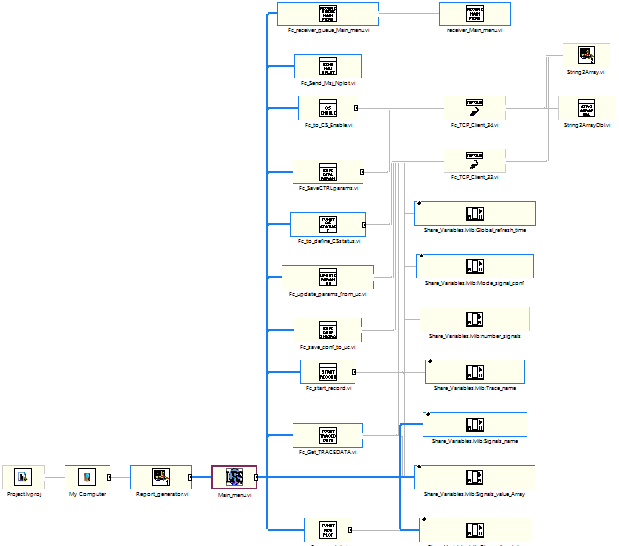
\includegraphics{LVtemp20240312184737_17_0h.png}

\hfill\break
Window\_plot.vi\\

\includegraphics{LVtemp20240312184738_0_0c.png}\\
This window has the capability to visualize and analyze the graphs of
the stored signals from the Main\_menu.\\
\strut \\
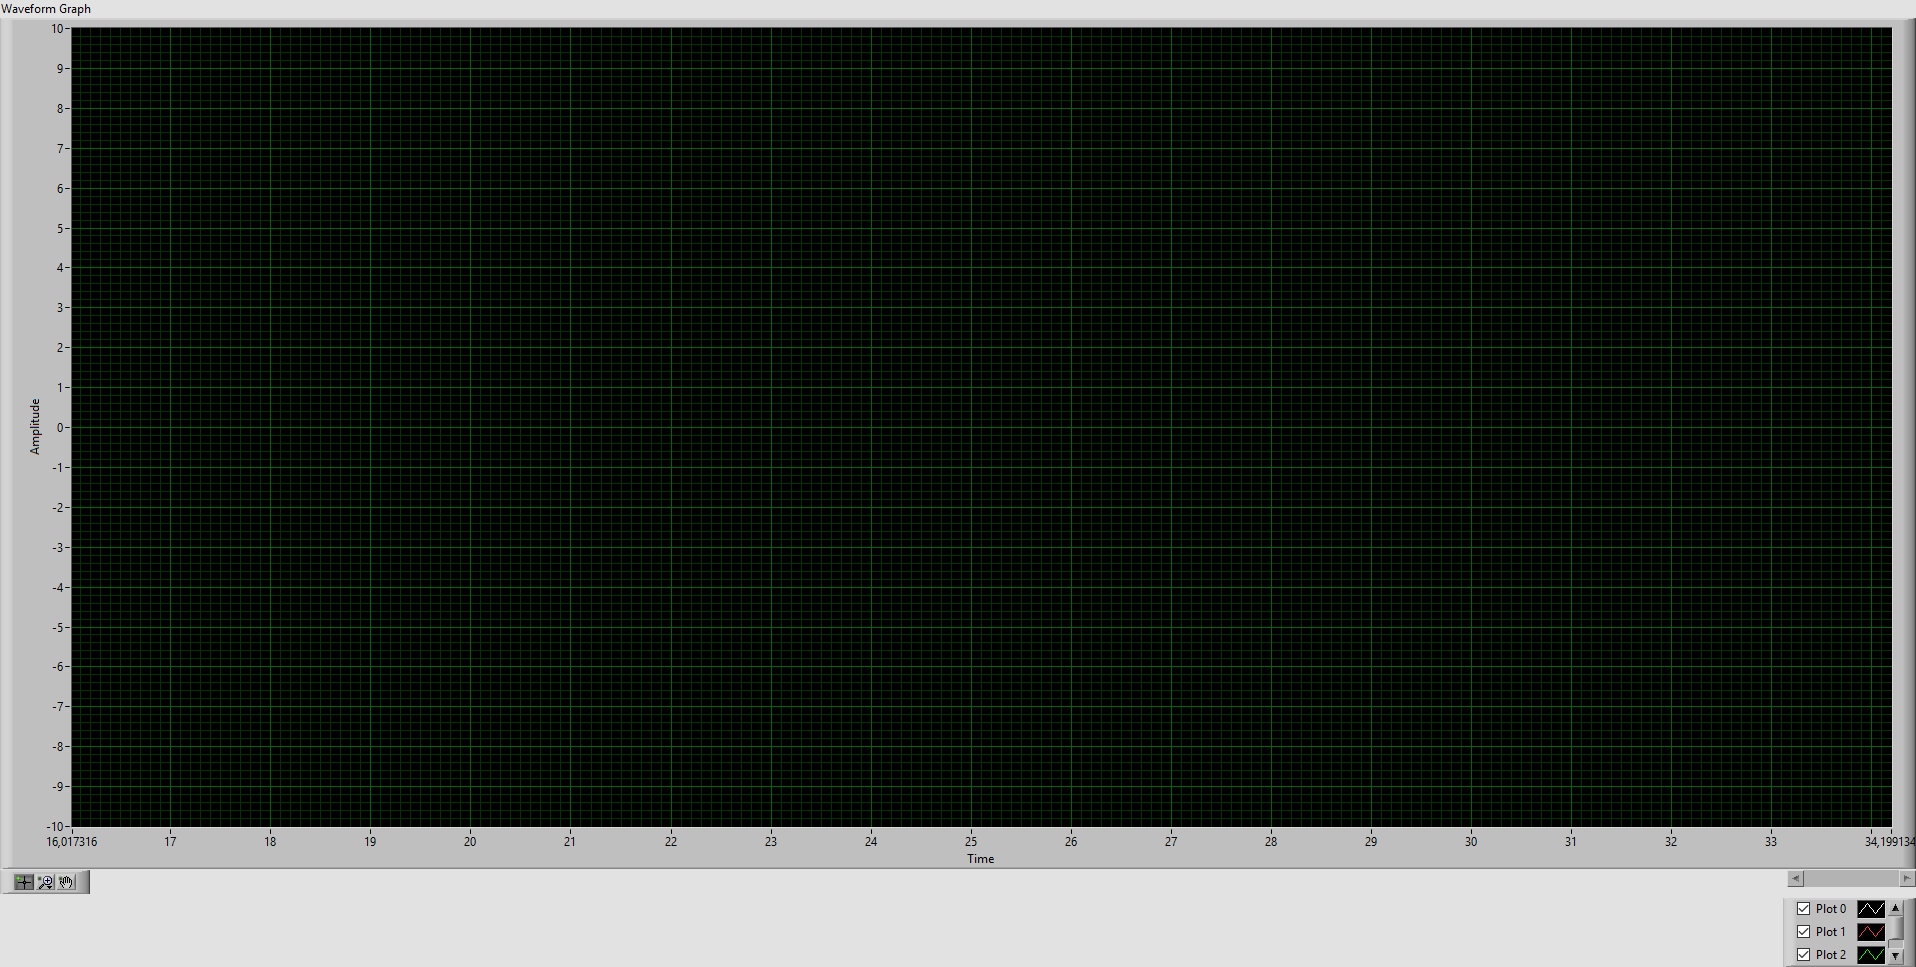
\includegraphics{LVtemp20240312184738_1_0.png}\\
\strut \\

\includegraphics{Fc_2update_graph_viLVtemp20240312184738_2_0.png}
\textbf{Fc\_2update\_graph.vi\\
}
C:\textbackslash Users\textbackslash v\_hernandez\textbackslash Documents\textbackslash Projects\textbackslash C2\textbackslash lrs-soc\textbackslash labview\textbackslash dev\_labview\textbackslash Fc\_2update\_graph.vi\\

\includegraphics{Fc_evaluate_state_viLVtemp20240312184738_3_0.png}
\textbf{Fc\_evaluate\_state.vi\\
}
C:\textbackslash Users\textbackslash v\_hernandez\textbackslash Documents\textbackslash Projects\textbackslash C2\textbackslash lrs-soc\textbackslash labview\textbackslash dev\_labview\textbackslash Fc\_evaluate\_state.vi\\

\includegraphics{Fc_MenuSelections_viLVtemp20240312184738_4_0.png}
\textbf{Fc\_MenuSelections.vi\\
}
C:\textbackslash Users\textbackslash v\_hernandez\textbackslash Documents\textbackslash Projects\textbackslash C2\textbackslash lrs-soc\textbackslash labview\textbackslash dev\_labview\textbackslash Fc\_MenuSelections.vi\\

\includegraphics{Fc_queue_receiver2Window_viLVtemp20240312184738_5_0.png}
\textbf{Fc\_queue\_receiver2Window.vi\\
}
C:\textbackslash Users\textbackslash v\_hernandez\textbackslash Documents\textbackslash Projects\textbackslash C2\textbackslash lrs-soc\textbackslash labview\textbackslash dev\_labview\textbackslash Fc\_queue\_receiver2Window.vi\\

\includegraphics{Simple_Error_Handler_viLVtemp20240312184738_6_0.png}
\textbf{Simple Error Handler.vi\\
} C:\textbackslash Program Files\textbackslash National
Instruments\textbackslash LabVIEW
2022\textbackslash vi.lib\textbackslash Utility\textbackslash error.llb\textbackslash Simple
Error Handler.vi\\

\hfill\break
Call\_signal\_fromHW.vi\\
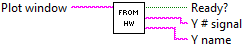
\includegraphics{LVtemp20240312184738_7_0c.png}\\
Through this function you can select the stored signals from the
Main\_menu.\\
\strut \\
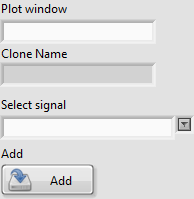
\includegraphics{LVtemp20240312184738_8_0.png}\\
\strut \\
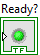
\includegraphics{LVtemp20240312184738_9_0.png} \textbf{Ready?\\
}\strut \\
\strut \\
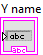
\includegraphics{LVtemp20240312184738_10_0.png} \textbf{Y name\\
}\strut \\
\strut \\
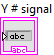
\includegraphics{LVtemp20240312184738_11_0.png} \textbf{Y \# signal\\
}\strut \\
\strut \\
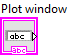
\includegraphics{LVtemp20240312184738_12_0.png} \textbf{Plot window\\
}\strut \\
\strut \\

\hfill\break
Call\_signal\_fromfile.vi\\
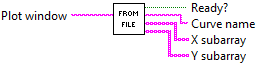
\includegraphics{LVtemp20240312184738_13_0c.png}\\
Through this function you can select the signals stored in a CSV file.\\
\strut \\
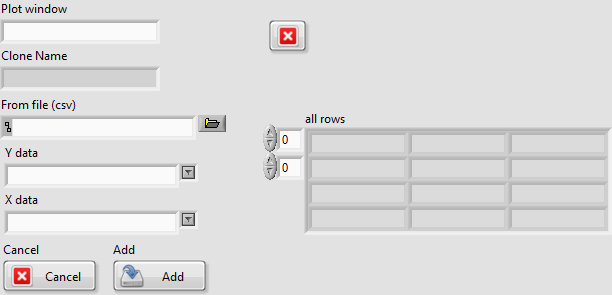
\includegraphics{LVtemp20240312184738_14_0.png}\\
\strut \\
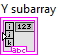
\includegraphics{LVtemp20240312184738_15_0.png} \textbf{Y subarray\\
}\strut \\
\strut \\

\begin{quote}
\hfill\break

String
\end{quote}

\hfill\break

\begin{quote}
\end{quote}

\hfill\break
\hfill\break
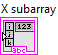
\includegraphics{LVtemp20240312184738_16_0.png} \textbf{X subarray\\
}\strut \\
\strut \\

\begin{quote}
\hfill\break

String
\end{quote}

\hfill\break

\begin{quote}
\end{quote}

\hfill\break
\hfill\break
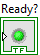
\includegraphics{LVtemp20240312184738_17_0.png} \textbf{Ready?\\
}\strut \\
\strut \\
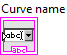
\includegraphics{LVtemp20240312184738_18_0.png} \textbf{Curve name\\
}\strut \\
\strut \\
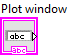
\includegraphics{LVtemp20240312184738_19_0.png} \textbf{Plot window\\
}\strut \\
\strut \\

\end{document}
